\section{Introducción}
% Especificar la motivación y las características principales del proyecto como así también un marco general
% sobre el estado del arte de la tecnología y el uso de las ideas o conceptos del proyecto propuesto.
En el ámbito universitario resulta necesario mantener informadas a las personas sobre una amplia variedad de hechos, noticias y acontecimientos que sucedieron o sucederán, desde la ubicación de un aula hasta la notificación de la cancelación de una clase. Muchas veces estas notificaciones son sobre cuestiones muy efímeras, lo que requiere rapidez para empezar a transmitirlas y facilidad para tener el alcance necesario.

En las facultades de la Universidad Nacional de La Plata se consumen muchos recursos para cumplir este fin, a través de afiches, pancartas, panfletos, etc. los cuales, pese a ser de barata fabricación, no tienen una vida útil muy extensa. Además todas estas formas de comunicacion se basan en el uso de papel, que tras ser utilizado debe desecharse debido a la imposibilidad de reutilizarlo, generando una cantidad de residuos significativa. Si se tiene en cuenta que también generan una polución visual considerable, por la gran cantidad de estos distribuidos en todos los lugares transitables, resulta prudente considerar una nueva forma de comunicación.

Surge así la idea de desarrollar de un cartel electrónico reutilizable, capaz de ser configurado remotamente por las autoridades competentes, con el fin de proveer una forma de comunicación masiva más limpia, clara y menos dañina para el medio ambiente. 

\section{Objetivos del proyecto}
% Deben especificarse los objetivos que se plantearon en el informe inicial
% (primarios y secundarios) se hayan cumplido o no (en las conclusiones se deberá contemplar
% el cambio de objetivos o el grado de cumplimiento de los mismos).
El objetivo principal del proyecto es implementar un cartel de LEDs que pueda ser configurado remotamente por un usuario.
El mismo se puede subdividir en subobjetivos, los cuales se mencionan a continuación:

Diseñar e implementar el Hardware (PCB, matrices de LEDs) del cartel para que visualice correctamente el mensaje configurado. Deberá ser modularizable, es decir, que sea posible agregar módulos funcionales y expandir la cantidad de caracteres en un renglón.

Desarrollar el software embebido que se ejecutará en el microcontrolador.

Desarrollar el software que controla el cartel. Éste podrá ser usado desde una pc y tendrá una interfaz gráfica con formato de panel para controlar las características del mensaje a mostrar por el cartel.

Diseñar e implementar protocolo de comunicación para la comunicación entre el software controlador del panel y el cartel. El protocolo debe establecer un método de autenticación que impida el acceso de personal no autorizado al cartel. Esto implica que sea seguro antes ataque del tipo \emph{man-in-the-middle} y otros tipos de ataques bien conocidos.

\section{Análisis de requerimientos}
% Enumerar los requerimientos funcionales y  no funcionales sobre los que se diseñó la solución propuesta.
% Especificar los aspectos funcionales que el sistema deberá cumplir respecto del usuario y su interacción con el mismo.



El panel proveerá una interfaz gráfica para que el usuario pueda configurar un mensaje para el cartel, así como modificar características secundarias como parpadeo, velocidad de movimiento o estaticidad del mensaje. A través del panel, el usuario podrá ingresar pore teclado el mensaje a mostrar mediante los caracteres que se establecen en el estándar (ver \cite{CodifChar}). Además, el panel permitirá relevar la configuración y el estado actual de lo que se está mostrando en el cartel. La autenticación correspondiente al ingreso al panel será verificada mediante el uso de un token de identificación.

El cartel contará con matrices de LEDs blancos que en conjunto y sintonía formarán las letras correspondientes al mensaje a transmitir, permitiendo mostrar el mensaje configurado por el usuario. 

El software compila ahre rama y agus vean esto

% Hablar de limites de tiempos (tiempo máximo de respuesta de conexión)

\section{Diseño del hardware}
% Describir el hardware propuesto, comenzando por un diagrama en bloques, luego una descripción de las Interfaces eléctricas
% (conexiones poncho-EDU-CIAA) y de usuario (teclado, displays, etc)
% hasta llegar al detalle fino de los componentes y circuitos a utilizar y sus características.
El cartel se compone de varios módulos. Cada módulo contiene una matriz de LED 8x8, un chip shifteador \cite{MAX7219}, y componentes pasivos varios, logrando así una unidad funcional independiente (ver figura \ref{fig:hw-moduloEsquematico}). 

\begin{figure}[ht!]
	\begin{center}
		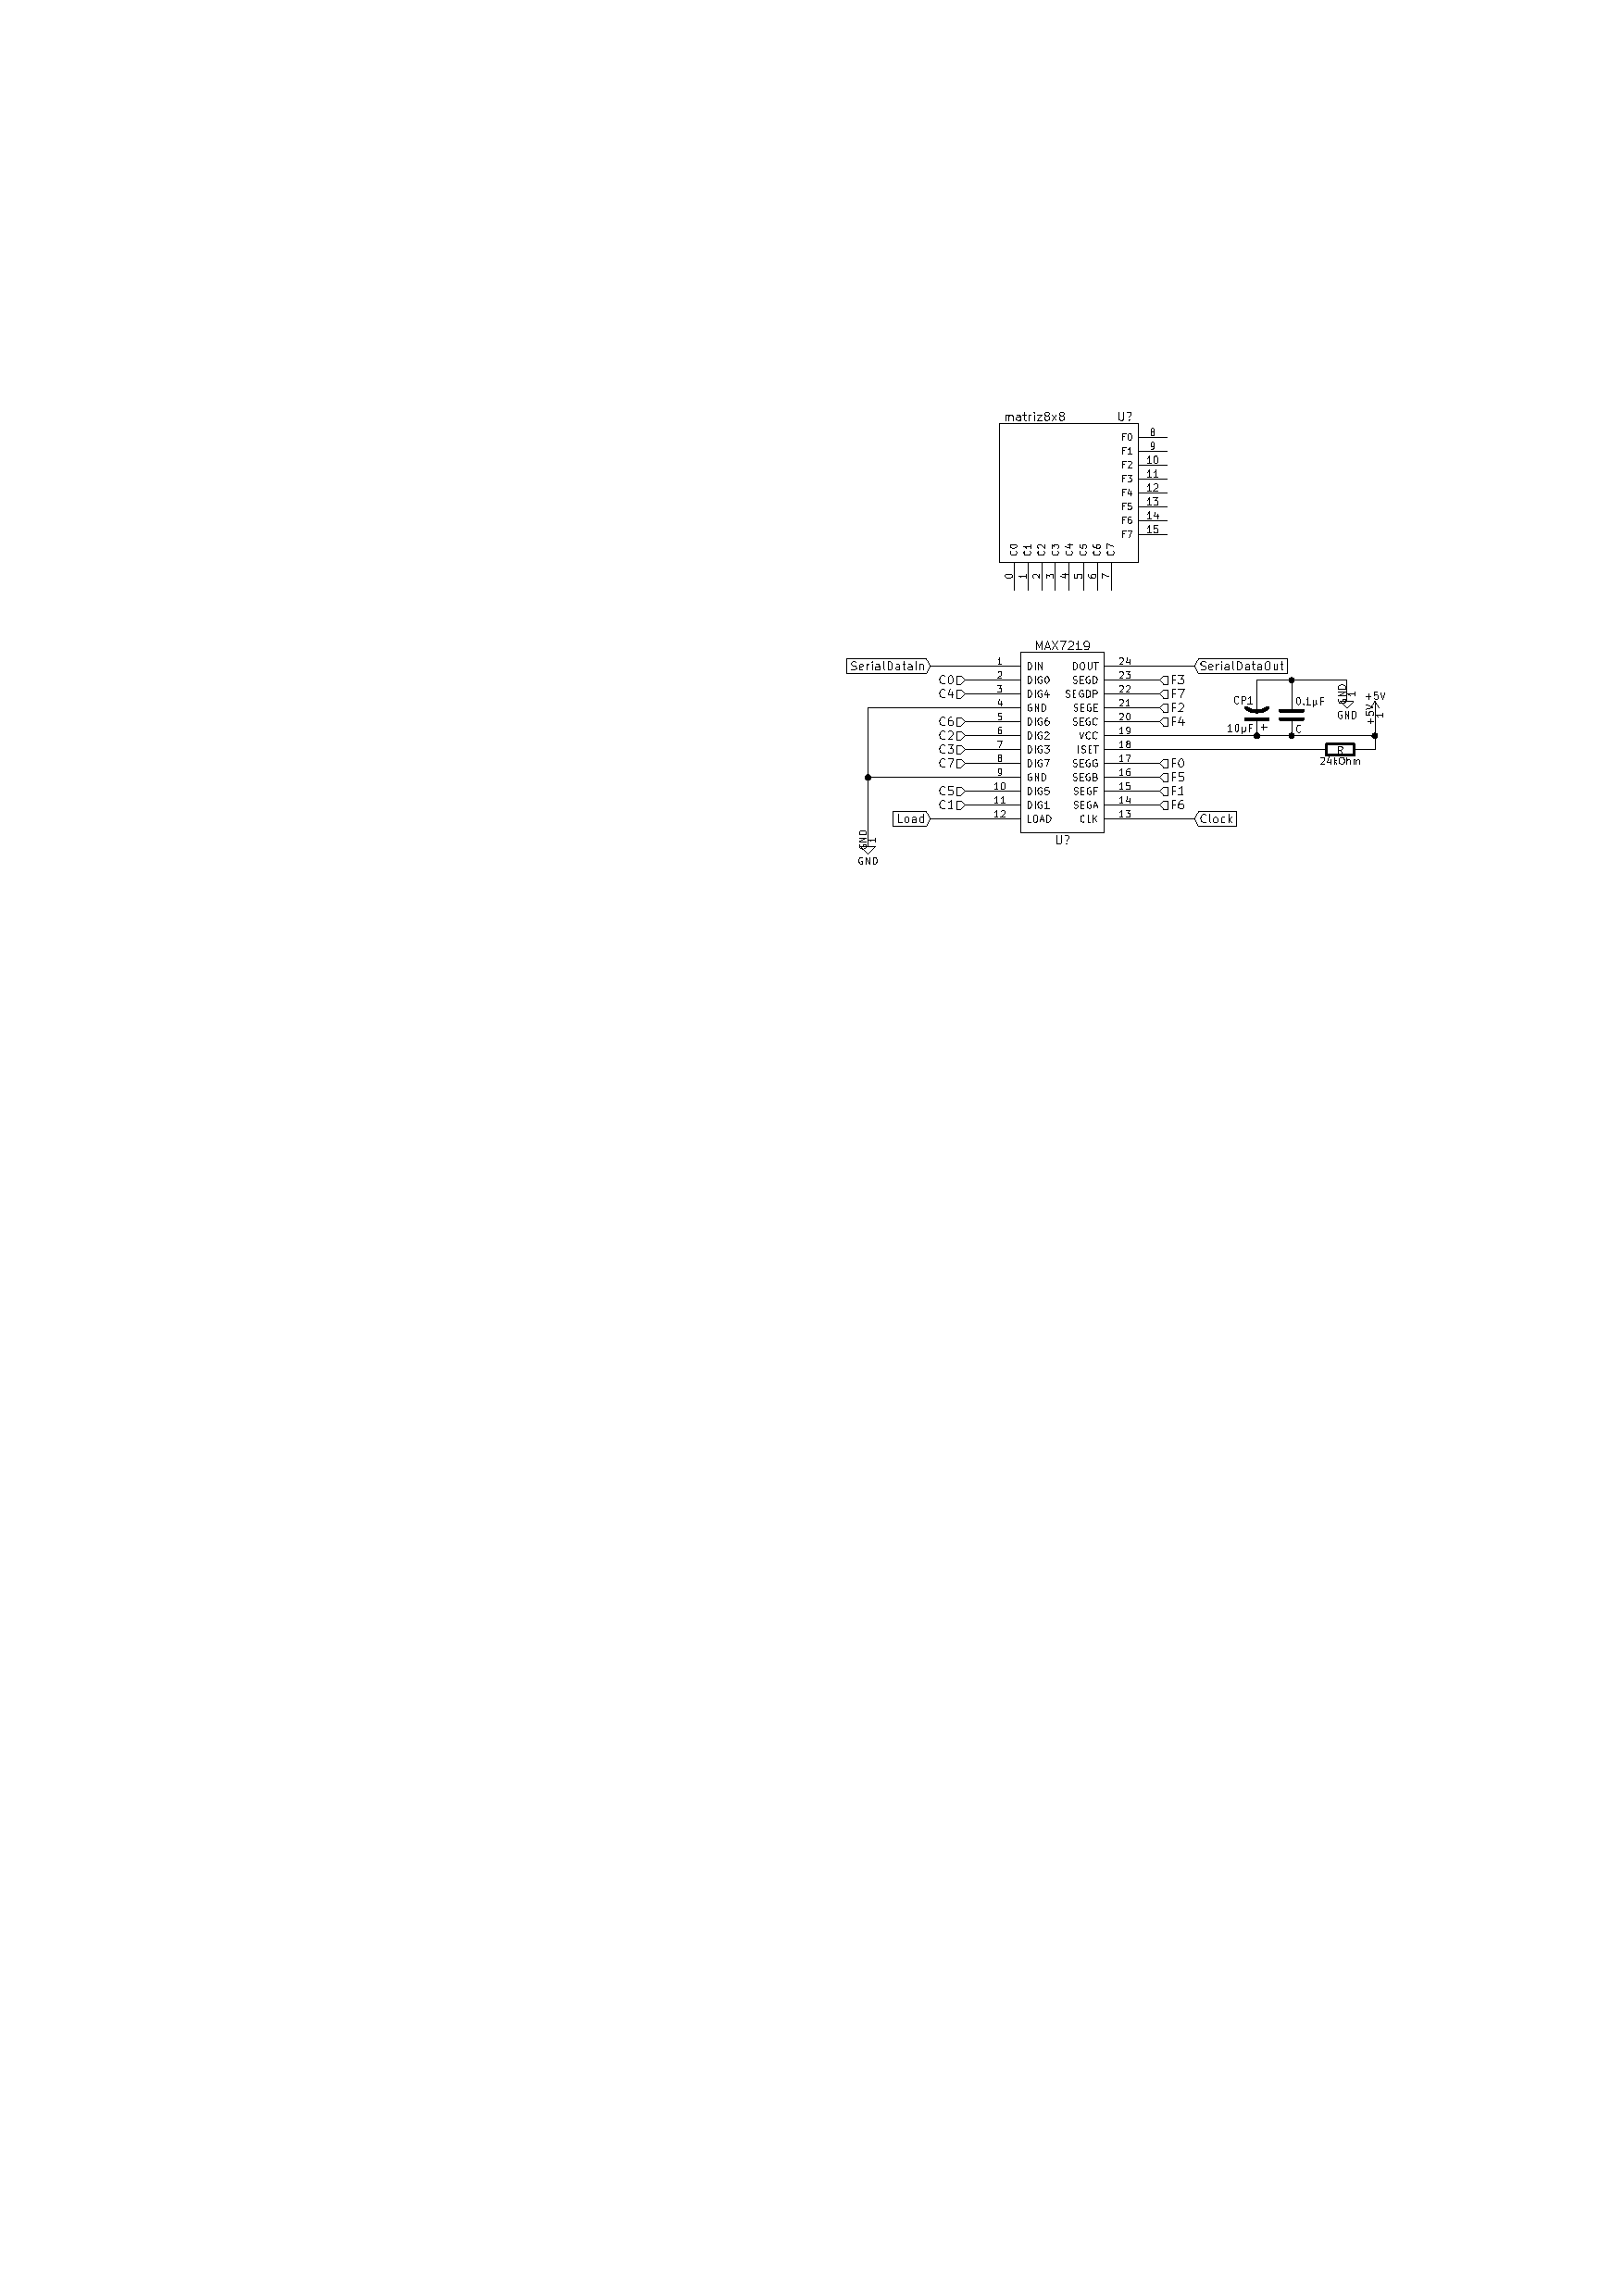
\includegraphics[width=0.8\textwidth]{imagenes/hw/moduloEsquematico}
		\caption{Esquema de conexiones de un módulo funcional.}
		\label{fig:hw-moduloEsquematico}
	\end{center}
\end{figure}


\begin{figure}[ht!]
	\begin{center}
		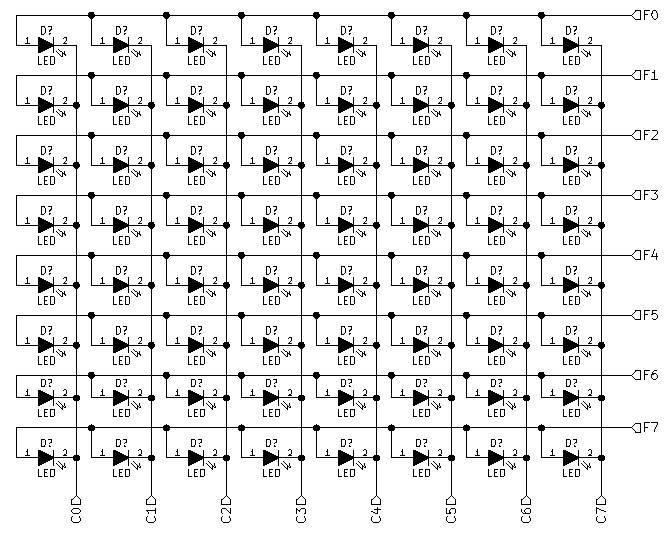
\includegraphics[width=0.7\textwidth]{imagenes/hw/moduloLED}
		\caption{Esquema de conexiones de un módulo funcional.}
		\label{fig:hw-moduloLED}
	\end{center}
\end{figure}

El MAX7219 recibe una secuencia de bytes de forma serial y los deriva a la columna que corresponda para cada instante en la matriz de LEDs del módulo correspondiente en el cartel. 

\section{Diseño de software}
% Descripción del software propuesto, comenzando por un diagrama de estados, pseudocódigo o esquemas que permitan
% comprender la arquitectura de software elegida (Controlada por eventos o por tiempo, apropiativa, cooperativa, etc).
% Luego especificar las diferentes módulos (o tareas) a implementar, drivers, bibliotecas a utilizar,
% prioridades y planificación de las distintas tareas (No incluir en el informe código C).
\subsection{Panel de configuración (PC)}
\subsection{Software embebido}


\section{Ensayos y mediciones}
% Describir el proceso de construcción del prototipo y los ensayos realizados para verificar el funcionamiento del mismo.
% Mostrar mediciones o resultados obtenidos en forma de tablas, figuras, 
% fotografías del sistema, pantallas de osciloscopios, pantallas de display, etc
Se desarrolló un prototipo de uno de los módulos funcionales del cartel, conectando los componentes sobre un protoboard y soldando una matriz de LEDs con la disposición a utilizar en el modelo final (ver Figura \ref{fig:hw-moduloLED}). A través del mismo se hicieron pruebas para corroborar el correcto funcionamiento particular de un módulo funcional y la claridad del carácter mostrado. Se corroboró que el mensaje comienza a mostrarse pocos instantes después de que el mismo empieza a ser recibido por el cartel. También se puso a prueba la tensión máxima soportada por los LEDs utilizados, los cuales demostraron la capacidad de soportar hasta 4,2 V de tensión con una corriente continua de 20 mA. En dicho prototipo se usaron resistencias que diferían levemente de las planteadas en el esquema original debido a problemas de disponibilidad de las mismas, confirmando que el módulo funciona correctamente con un margen de tolerancia para los valores de tensión y corriente en los LEDs. El prototipo también permitió confirmar que el sistema puede prescindir de un disipador térmico ya que los componentes no levantan una temperatura considerable, aún después de un funcionamiento prolongado.


\section{Conclusiones parciales}
% 1-Explicar el grado de avance de los objetivos planteados hasta el momento como así también el trabajo a seguir.
% 2-Describir claramente la actividad de cada integrante del grupo, evaluar las horas invertidas hasta el momento
%	y re-estimar las horas de ingeniería restantes.
% 3- Evaluar y destacar correcciones o desvíos del cronograma de tareas presentado en el informe de inicial.
% 4-Analizar el presupuesto invertido y corregir (si corresponde) el presupuesto final del proyecto. 

Se corroboró que la implementación práctica de la matriz de LEDs usando el esquema planteado originalmente permite mostrar correctamente el mensaje que el usuario disponga.

Se diseñó un protocolo para la comunicación entre el panel de configuración y el cartel.

Nahuel Ternouski y Santiago Levy plantearon el esquema de hardware y desarrollaron el prototipo del módulo funcional.

% Agustín García y Ramiro Romero Dapozo desarrollaron algo qcyo

Nahuel Ternouski y Ramiro Romero Dapozo desarrollaron la interfaz del panel a utilizar para que el usuario configure el mensaje.

El desarrollo de las actividades viene cumpliendo satisfactoriamente con los tiempos del cronograma estipulado.

Hasta el momento el presupuesto invertido por los alumnos en el proyecto para el desarrollo del prototipo de un módulo funcional ronda los 500 pesos.